%%%%%% -*- Coding: utf-8-unix; Mode: latex

%\documentclass[polish]{projectreport}
\documentclass[english]{projectreport}

\usepackage[utf8]{inputenc}
\usepackage{url}
\usepackage{subfigure}
\usepackage{tabularx}
\usepackage{ragged2e}
\usepackage{booktabs}
\usepackage{multirow}
\usepackage{grffile}

\usepackage[bookmarks=false]{hyperref}
\hypersetup{colorlinks,
  linkcolor=blue,
  citecolor=blue,
  urlcolor=blue}

\usepackage{indentfirst}
\usepackage{caption}
\usepackage{listings}
\usepackage[ruled,linesnumbered,lined]{algorithm2e}
\usepackage[svgnames]{xcolor}
\usepackage{inconsolata}
\usepackage{fancyhdr}

\usepackage{csquotes}
\DeclareQuoteStyle[quotes]{polish}
  {\quotedblbase}
  {\textquotedblright}
  [0.05em]
  {\quotesinglbase}
  {\fixligatures\textquoteright}
\DeclareQuoteAlias[quotes]{polish}{polish}

\usepackage[
style=numeric,
sorting=nyt,
isbn=false,
doi=true,
url=true,
backref=false,
backrefstyle=none,
maxnames=10,
giveninits=true,
abbreviate=true,
defernumbers=false,
backend=biber]{biblatex}
\addbibresource{bibliography.bib}

\lstset{
    %language=Python, %% PHP, C, Java, etc.
    basicstyle=\ttfamily\footnotesize,
    backgroundcolor=\color{gray!5},
    commentstyle=\it\color{Green},
    keywordstyle=\color{Red},
    stringstyle=\color{Blue},
    numberstyle=\tiny\color{Black},    
    % morekeywords={TestKeyword},
    % mathescape=true,
    escapeinside=`',
    frame=single, %shadowbox, 
    tabsize=2,
    rulecolor=\color{black!30},
    title=\lstname,
    breaklines=true,
    breakatwhitespace=true,
    framextopmargin=2pt,
    framexbottommargin=2pt,
    extendedchars=false,
    captionpos=b,
    abovecaptionskip=5pt,
    keepspaces=true,            
    numbers=left,                    
    numbersep=5pt,                  
    showspaces=false,                
    showstringspaces=false,
    showtabs=false,
    tabsize=2
}

\SetAlgorithmName{\LangAlgorithm}{\LangAlgorithmRef}{\LangListOfAlgorithms}

\renewcommand{\lstlistingname}{\LangListing}
\renewcommand\lstlistlistingname{\LangListOfListings}

\newcolumntype{Y}{>{\small\centering\arraybackslash}X}
%\newcolumntype{b}{>{\hsize=1.6\hsize}Y}
%\newcolumntype{m}{>{\hsize=.6\hsize}Y}
%\newcolumntype{s}{>{\hsize=.4\hsize}Y}

\captionsetup[figure]{skip=5pt,position=bottom}
\captionsetup[table]{skip=5pt,position=top}



%%%%%%%%%%%%%%%%%%%%%%%%%%%%%%%%%%%%%%%%%%%%%%%%%%%%%%%%%%%%%%%%%%%%%%%%%%%%%%%
\author{Przemysław Popowski$^1$}

\title{Predator-prey coevolution simulation}

\date{
	{\small $^1$AGH Krakow \\ \texttt{popowskip@student.agh.edu.pl}\\[1ex]%
        \the\year}
      }
      
\pagestyle{fancy}
\fancyhf{}
\fancyhead[LE,RO]{\thepage}

%%%%%%%%%%%%%%%%%%%%%%%%%%%%%%%%%%%%%%%%%%%%%%%%%%%%%%%%%%%%%%%%%%%%%%%%%%%%%%%
\begin{document}

\maketitle

\thispagestyle{empty}

\begin{abstract}
\noindent Understanding predator-prey dynamics is essential for ecological research, but traditional mathematical models often fail to capture the complexities of interactions, individual behaviors, and random chance. This paper presents an agent-based model developed in Python to simulate a virtual ecosystem with grass, prey, and predators. By assigning energy costs to actions such as movement and reproduction, the simulation provides a realistic, individual representation of survival and population cycles. Furthermore, each agent carries an evolvable genotype; offspring inherit their parent's genes with random Gaussian mutations, driving a co-evolutionary arms race between predators and prey without any pre-programmed target behavior. The project features a fully functional visual environment coupled with a user-friendly control panel, allowing users to dynamically adjust ecological parameters and save scenarios without requiring programming expertise. The primary objectives are to observe ecosystem stability, extinction events, and "boom and bust" population cycles under varied conditions.

\vspace*{0.5em}
\noindent\textbf{Keywords:} agent-based modeling, predator-prey dynamics, ecosystem simulation, population dynamics, Python, visual environment, configurable ecological research
\end{abstract}

%%%%%%%%%%%%%%%%%%%%%%%%%%%%%%%%%%%%%%%%%%%%%%%%%%%%%%%%%%%%%%%%%%%%%%%%%%%%%%%
\section{Project Overview: Simulating the Circle of Life}
\label{sec:introduction}

\subsection{The Background}
In nature, the relationship between predators and their prey is a delicate balancing act. When prey populations (such as rabbits) grow, predators (such as foxes) have more food and multiply. When predators eat too much, food runs out, and their numbers drop. For a long time, scientists used mathematical equations to study these cycles. While those equations were a great starting point, they had a major flaw: they treated animals as perfectly mixed numbers on a page. They did not account for real factors such as physical space, the effort required to hunt, or simple random chance.

\subsection{The Modern Approach: Virtual Ecosystems}
To get a more realistic picture, modern researchers use "agent-based models". Instead of using abstract math, this approach works a bit like a video game, creating a virtual world filled with independent, autonomous agents. Due to its flexibility, agent-based modeling has become a widely used tool in many fields. In evolutionary modeling, it has been applied to the mechanisms of sexual selection and pair formation \cite{drezewski2018}, including individual-based quantitative-genetic simulations \cite{dijk2010}.

In ecological contexts, agent-based models enable the study of predator-prey coevolution in physically simulated environments. Previous work has demonstrated how predator and prey populations co-evolve through adaptation \cite{ouannes2015, takashi2013}. Furthermore, Van der Laan and Hogeweg \cite{vanderlaan1995} showed how ecological and evolutionary dynamics can interact across different timescales.

More recently, these models have been extended by incorporating artificial intelligence techniques. Reinforcement learning, for example, has been used to study the co-evolution of predator-prey ecosystems in which agents actively adapt their strategies \cite{park2021}. Similarly, predator-induced survival pressure alone has been shown to lead to the emergence of complex collective behaviors such as swarming \cite{li2023}.

\subsection{What This Project Does}
Following this modern and open approach, this project focuses on building an agent-based simulation of a simple food chain. It includes three levels:
\begin{itemize}
\item \textbf{Grass} that slowly grows back over time.
\item \textbf{Prey} that wander around eating the grass.
\item \textbf{Predators} that hunt prey.
\end{itemize}

Every action an animal takes costs energy, and the only way they can survive is by finding food.

\noindent \textbf{The main goals of this project are:}
\begin{itemize}
    \item To build a working, easy-to-use computer simulation of this predator-prey relationship.
    \item To test what happens when we tweak the rules of nature. For example, what happens if grass grows slower? What if predators need more food to survive?
    \item To see if our virtual world ends in a stable balance, constant population rollercoasters, or total extinction.
    \item To explore how individual agent rules lead to complex, ecosystem-wide consequences, drawing inspiration from modern computational studies.
\end{itemize}

\subsection{What Was Built}
To make this happen, the project includes the following:
\begin{itemize}
    \item \textbf{A fully functioning virtual environment} programmed in Python that acts as a visual grid where animals move and interact.
    \item \textbf{An explicit ecosystem} where grass grows continuously, prey consume grass, and predators consume prey.
    \item \textbf{A gene-driven energy system} where traits like metabolism and reproduction evolve dynamically from user-defined starting parameters.
    \item \textbf{A user-friendly control panel} that lets users easily change the simulation's settings and save their favorite scenarios without needing to code.
    \item \textbf{A genetic evolution system} where random mutations at birth drive ongoing predator-prey coevolution purely through natural survival.
    \item \textbf{A live analytics dashboard} featuring real-time population charts, death statistics by cause, and point-and-click genotype inspection.
\end{itemize}
%%%%%%%%%%%%%%%%%%%%%%%%%%%%%%%%%%%%%%%%%%%%%%%%%%%%%%%%%%%%%%%%%%%%%%%%%%%%%%%
%%%%%%%%%%%%%%%%%%%%%%%%%%%%%%%%%%%%%%%%%%%%%%%%%%%%%%%%%%%%%%%%%%%%%%%%%%%%%%%
\section{Problem formulation and proposed solution}
\label{sec:problem}

This section formalises the research problem and details the proposed simulation, building upon the motivation and literature review from Section 1. The following subsections describe the system architecture (\ref{sec:architecture}), the formal equations governing agent interactions (\ref{sec:equations}), and the core step dynamics alongside the genetic mutation scheme (\ref{sec:algorithms}).

\subsection{Research problem formulation}
\label{sec:problem-formulation}

Classical differential equation models, such as the Lotka–Volterra system, assume populations are continuous and perfectly mixed. While useful for basic analysis, they fail to capture spatial structure, individual variation, and the randomness of local interactions \cite{vanderlaan1995}.

This project addresses these limitations. The core research question is: \textbf{How do population-level dynamics emerge from the purely local interactions of individual prey and predators, each possessing an evolvable genotype?}

Specifically, the study investigates:
\begin{itemize}
    \item Under which parameter conditions does the ecosystem stabilise, oscillate, or collapse?
    \item What specific genetic traits does natural selection favour for each species?
    \item Can different survival strategies (e.g., living longer with a low metabolism vs.\ living shorter but reproducing rapidly) emerge spontaneously, without being explicitly programmed \cite{takashi2013}?
\end{itemize}

\paragraph{Proposed solution.} To answer these questions, an agent-based simulation implemented in Python is proposed. The environment is a 2D grid with wrap-around edges (a torus), populated by three interacting entities: grass cells, prey, and predators. Unlike classical models, every animal carries a unique genotype. When animals reproduce, their genes mutate via multiplicative Gaussian noise, following the quantitative-genetic approach of \cite{dijk2010}. This mechanism drives continuous predator–prey coevolution based solely on local survival and reproduction pressures \cite{takashi2013, ouannes2015, li2023}.

\subsection{System architecture}
\label{sec:architecture}

The system is built around three distinct logical layers, following the single-responsibility principle:

\begin{itemize}
    \item \textbf{Configuration layer.} A \texttt{pygame\_gui}-based setup interface (\texttt{config\_screen.py}) where the user adjusts initial parameters (population sizes, mutation bounds, gene values) and selects saved scenarios. Configurations are saved as JSON files.
    \item \textbf{Simulation engine.} The core logic, encapsulated within the \texttt{Simulation} class \\ (\texttt{simulation.py}). At each time step, it updates grass growth and handles all animal interactions: movement, feeding, reproduction, ageing, and death.
    \item \textbf{Renderer and analytics.} Managed by the \texttt{SimRenderer} class, this layer handles the visual output. It draws the 2D spatial grid and updates the interactive side-panel with real-time charts, death statistics, and genetic data. Users can also click on any agent to inspect its exact genes.
\end{itemize}

External data is kept separate from the main codebase: parameter definitions are in \\ \texttt{configs/parameters/default.json}, UI layouts in \texttt{configs/layout.json}, and gene descriptions in \texttt{configs/genes\_info.json}. This clean separation makes it easy to maintain the code, run reproducible experiments, and test different ecological scenarios.


\subsection{Simulation mechanics}
\label{sec:equations}

The simulation operates on a toroidal (wrap-around) 2D grid. Each animal has a state consisting of its position, energy, age, and a dictionary of genes. The rules described below directly reflect the logic implemented in the Python engine.

\paragraph{Movement.} An animal chooses a random direction from the 8 neighboring cells. The number of cells it actually moves ($n$) depends on its \texttt{move\_distance} gene $d$:
\begin{equation}
n = \max(1,\; \lfloor d \rfloor + X)
\label{eq:cells_moved}
\end{equation}
where $X = 1$ with probability $d - \lfloor d \rfloor$, and $0$ otherwise. This allows fractional gene values to translate into discrete grid steps (e.g., a distance of $1.7$ means $1$ step plus a $70\%$ chance for a second step). Movement drains energy based on the distance:
\begin{equation}
E_{\text{new}} = E_{\text{old}} - (\texttt{move\_cost} \cdot n)
\label{eq:move_cost}
\end{equation}

\paragraph{Encounters and feeding.} If a predator and a prey occupy the same cell, the predator catches the prey with the following probability:
\begin{equation}
P(\text{catch}) = \texttt{hunt\_success} \cdot (1 - \texttt{escape\_chance})
\label{eq:catch}
\end{equation}
If successful, the prey dies immediately, and the predator gains energy (capped at its maximum):
\begin{equation}
E_{\text{new}} = \min(\texttt{max\_energy},\; E_{\text{old}} + \texttt{eat\_energy})
\label{eq:eat}
\end{equation}
Prey eat from their current cell whenever the local grass level exceeds $0.2$; a successful meal reduces the cell's grass by $0.4$ and grants the prey \texttt{eat\_energy} energy (capped at \texttt{max\_energy}).

\paragraph{Ageing and death.} Once an animal's age exceeds its \texttt{max\_age} gene, it faces a growing probability of natural death per step:
\begin{equation}
P(\text{death}) = \min\left(1,\; 0.05 \cdot \left(\frac{\text{age}}{\texttt{max\_age}} - 1\right)\right)
\label{eq:senescence}
\end{equation}

\paragraph{Reproduction.} If an animal's energy is at least \texttt{reproduce\_energy}, it attempts to reproduce with a probability equal to its \texttt{reproduce\_chance} gene. If successful, the parent transfers a fraction of its energy to the newborn child:
\begin{equation}
E_{\text{child}} = \lfloor E_{\text{parent}} \cdot \texttt{offspring\_investment} \rfloor
\label{eq:reproduce}
\end{equation}
The parent's energy is reduced by exactly $E_{\text{child}}$ to ensure strict energy conservation within the ecosystem.

\paragraph{Genetic mutation.} A newborn inherits its parent's genes, but a random number of them (between \texttt{mutation\_min} and \texttt{mutation\_max}) undergo mutation. Each selected gene is multiplied by a Gaussian random variable:
\begin{equation}
g_{\text{new}} = \max\left(0,\; g_{\text{old}} \cdot \bigl(1 + N(0, \sigma)\bigr)\right)
\label{eq:mutation}
\end{equation}
where $N(0, \sigma)$ is a normal distribution with mean $0$ and standard deviation $\sigma$ (\texttt{mutation\_strength}). Genes representing probabilities (like \texttt{escape\_chance} or \texttt{reproduce\_chance}) are additionally capped at $1.0$.

\paragraph{Metabolism.} Regardless of the actions taken, every animal pays a baseline metabolic cost at each time step to sustain its life functions. This is subtracted continuously:
\begin{equation}
E_{\text{new}} = E_{\text{old}} - \texttt{metabolism}
\label{eq:metabolism}
\end{equation}
If an animal's energy drops to zero or below as a result of movement or metabolism, it dies of starvation.


\subsection{Algorithms}
\label{sec:algorithms}

The genetic mutation mechanics described in Equation~(\ref{eq:mutation}) are implemented directly in Python, as shown in Listing~\ref{lst:mutate}. The function selects a random subset of genes and applies the multiplicative Gaussian noise, ensuring that probability-based traits remain correctly bounded within the $[0, 1]$ range.

\begin{lstlisting}[language=Python, caption={Multiplicative Gaussian mutation applied to an offspring's genes. Source: own work.}, label=lst:mutate]
def mutate_genes(parent_genes, cfg):
    child = dict(parent_genes)
    n_min = int(cfg["mutation_min"])
    n_max = int(cfg["mutation_max"])
    strength = cfg["mutation_strength"]
    n = random.randint(min(n_min, n_max), max(n_min, n_max))
    if n > 0:
        keys = random.sample(list(child.keys()), min(n, len(child)))
        for k in keys:
            child[k] = max(0.0, child[k] * (1 + random.gauss(0, strength)))
    # probability-valued genes clamped to [0, 1]
    for k in ("reproduce_chance", "escape_chance",
              "hunt_success", "offspring_investment"):
        if k in child:
            child[k] = min(1.0, child[k])
    return child
\end{lstlisting}

The overall progression of the ecosystem is driven by the engine's \texttt{step()} method. To provide a clear overview of the system's dynamics, Algorithm~\ref{alg:step} outlines the high-level logical flow of a single simulation tick, focusing on the core ecological rules rather than technical details like spatial indexing.


\begin{algorithm}[H]
\KwIn{simulation state (grass grid, animal population), configuration}
\KwOut{updated simulation state}
\BlankLine

Regrow grass uniformly across all grid cells\;
Build spatial index of currently alive animals\;

\ForEach{alive animal $a$ in the population}{
  Move $a$ by random direction and distance $n_a$ (Eq.~\ref{eq:cells_moved}--\ref{eq:move_cost})\;
  Increase age and evaluate natural senescence (Eq.~\ref{eq:senescence})\;
  
  \If{$a$ survives}{    
    \If{$a$ is prey}{
      Eat grass at current cell if available (Eq.~\ref{eq:eat})\;
      Deduct baseline metabolic cost $\mu_a$\;
      \If{predator $p$ is present \KwSty{and} $U(0,1) < P(\text{catch})$ (Eq.~\ref{eq:catch})}{
        $p$ gains energy; mark $a$ as dead\;
      }
    } \Else{
      Deduct baseline metabolic cost $\mu_a$\;
      \If{prey $q$ is present \KwSty{and} $U(0,1) < P(\text{catch})$}{
        $a$ gains energy; mark $q$ as dead\;
      }
    }
    
    \If{energy $\ge \theta_a$ \KwSty{and} $U(0,1) < r_a$}{
      Generate offspring with mutated genotype $\mathbf{g}_{\mathrm{child}}$ (Eq.~\ref{eq:mutation})\;
    }
  }
}

Remove dead or starved animals from the population\;
Integrate newborns into the population\;
Log aggregated population statistics\;

\caption{Description of a single simulation step.}
\label{alg:step}
\end{algorithm}



\subsection{Libraries and tooling}
\label{sec:tooling}

The implementation relies on a small set of well-established Python libraries:
\begin{itemize}
    \item \textbf{pygame 2.6} - the visual rendering backend and the input/event loop. Visual elements like cells, animals, and the chart are drawn using standard \texttt{pygame.draw} functions.
    \item \textbf{pygame\_gui} - handles UI widgets for the configuration screen and the analytics panel (labels, buttons, text fields, dropdowns). It also automatically manages styling, such as highlighting the active tab.
    \item \textbf{Python standard library} - \texttt{random} for random events and mutations, \\ \texttt{collections.deque} for history buffers, \texttt{json} for loading/saving configurations, and \texttt{csv} as a planned data export format.
\end{itemize}

No external numerical or machine-learning libraries are used. All simulation logic is written in plain Python using standard lists and dictionaries. This keeps the model completely transparent and easy to modify, at the cost of larger simulations being CPU-bound.



%%%%%%%%%%%%%%%%%%%%%%%%%%%%%%%%%%%%%%%%%%%%%%%%%%%%%%%%%%%%%%%%%%%%%%%%%%%%%%%
\section{Experimental research results}
\label{sec:results}

This section details the simulation's behavior under controlled conditions and addresses the research questions posed in Section~\ref{sec:problem-formulation}. The model was evaluated by directly observing the simulation via an interactive application - its configuration screen and live view are shown in Figures~\ref{fig:config} and~\ref{fig:sim}.

\subsubsection{Experimental setup.}
The simulation operates using the project's default configuration parameters. The environment consists of a $60 \times 40$ toroidal grid with a grass regrowth rate of $0.03$. The initial population is set to $80$ prey and $20$ predators. The model also utilizes the default gene values detailed on the application's \emph{Genes} tab. Each simulation run lasts for $1500$ steps, which provides sufficient time to observe several full population cycles.


\subsection{Figures and tables}
\label{sec:figs-tables}

\subsubsection{Figures}
\label{sec:figures}

Figure~\ref{fig:config} shows the configuration screen for managing ecological parameters and scenarios. Figure~\ref{fig:sim} illustrates the simulation during two characteristic phases: a prey boom with heavily grazed grass Figure~\ref{fig:sim} (a), followed by a predator boom that causes a prey collapse and allows grass recovery Figure~\ref{fig:sim} (b). The accompanying side panel displays real-time statistics, including population charts, death causes, and average genotypes.

The dynamics of the ecosystem are captured in three key plots. Figure~\ref{fig:popdyn} highlights the boom-and-bust nature of the system through a representative population time series. Figure~\ref{fig:genes} tracks the average values of genes over time, demonstrating the action of evolutionary selection on agents. Finally, Figure~\ref{fig:scenarios} compares population dynamics across three pre-configured scenarios to illustrate how different initial settings alter the simulation's behavior.

\begin{figure}[ht]
  \centering
  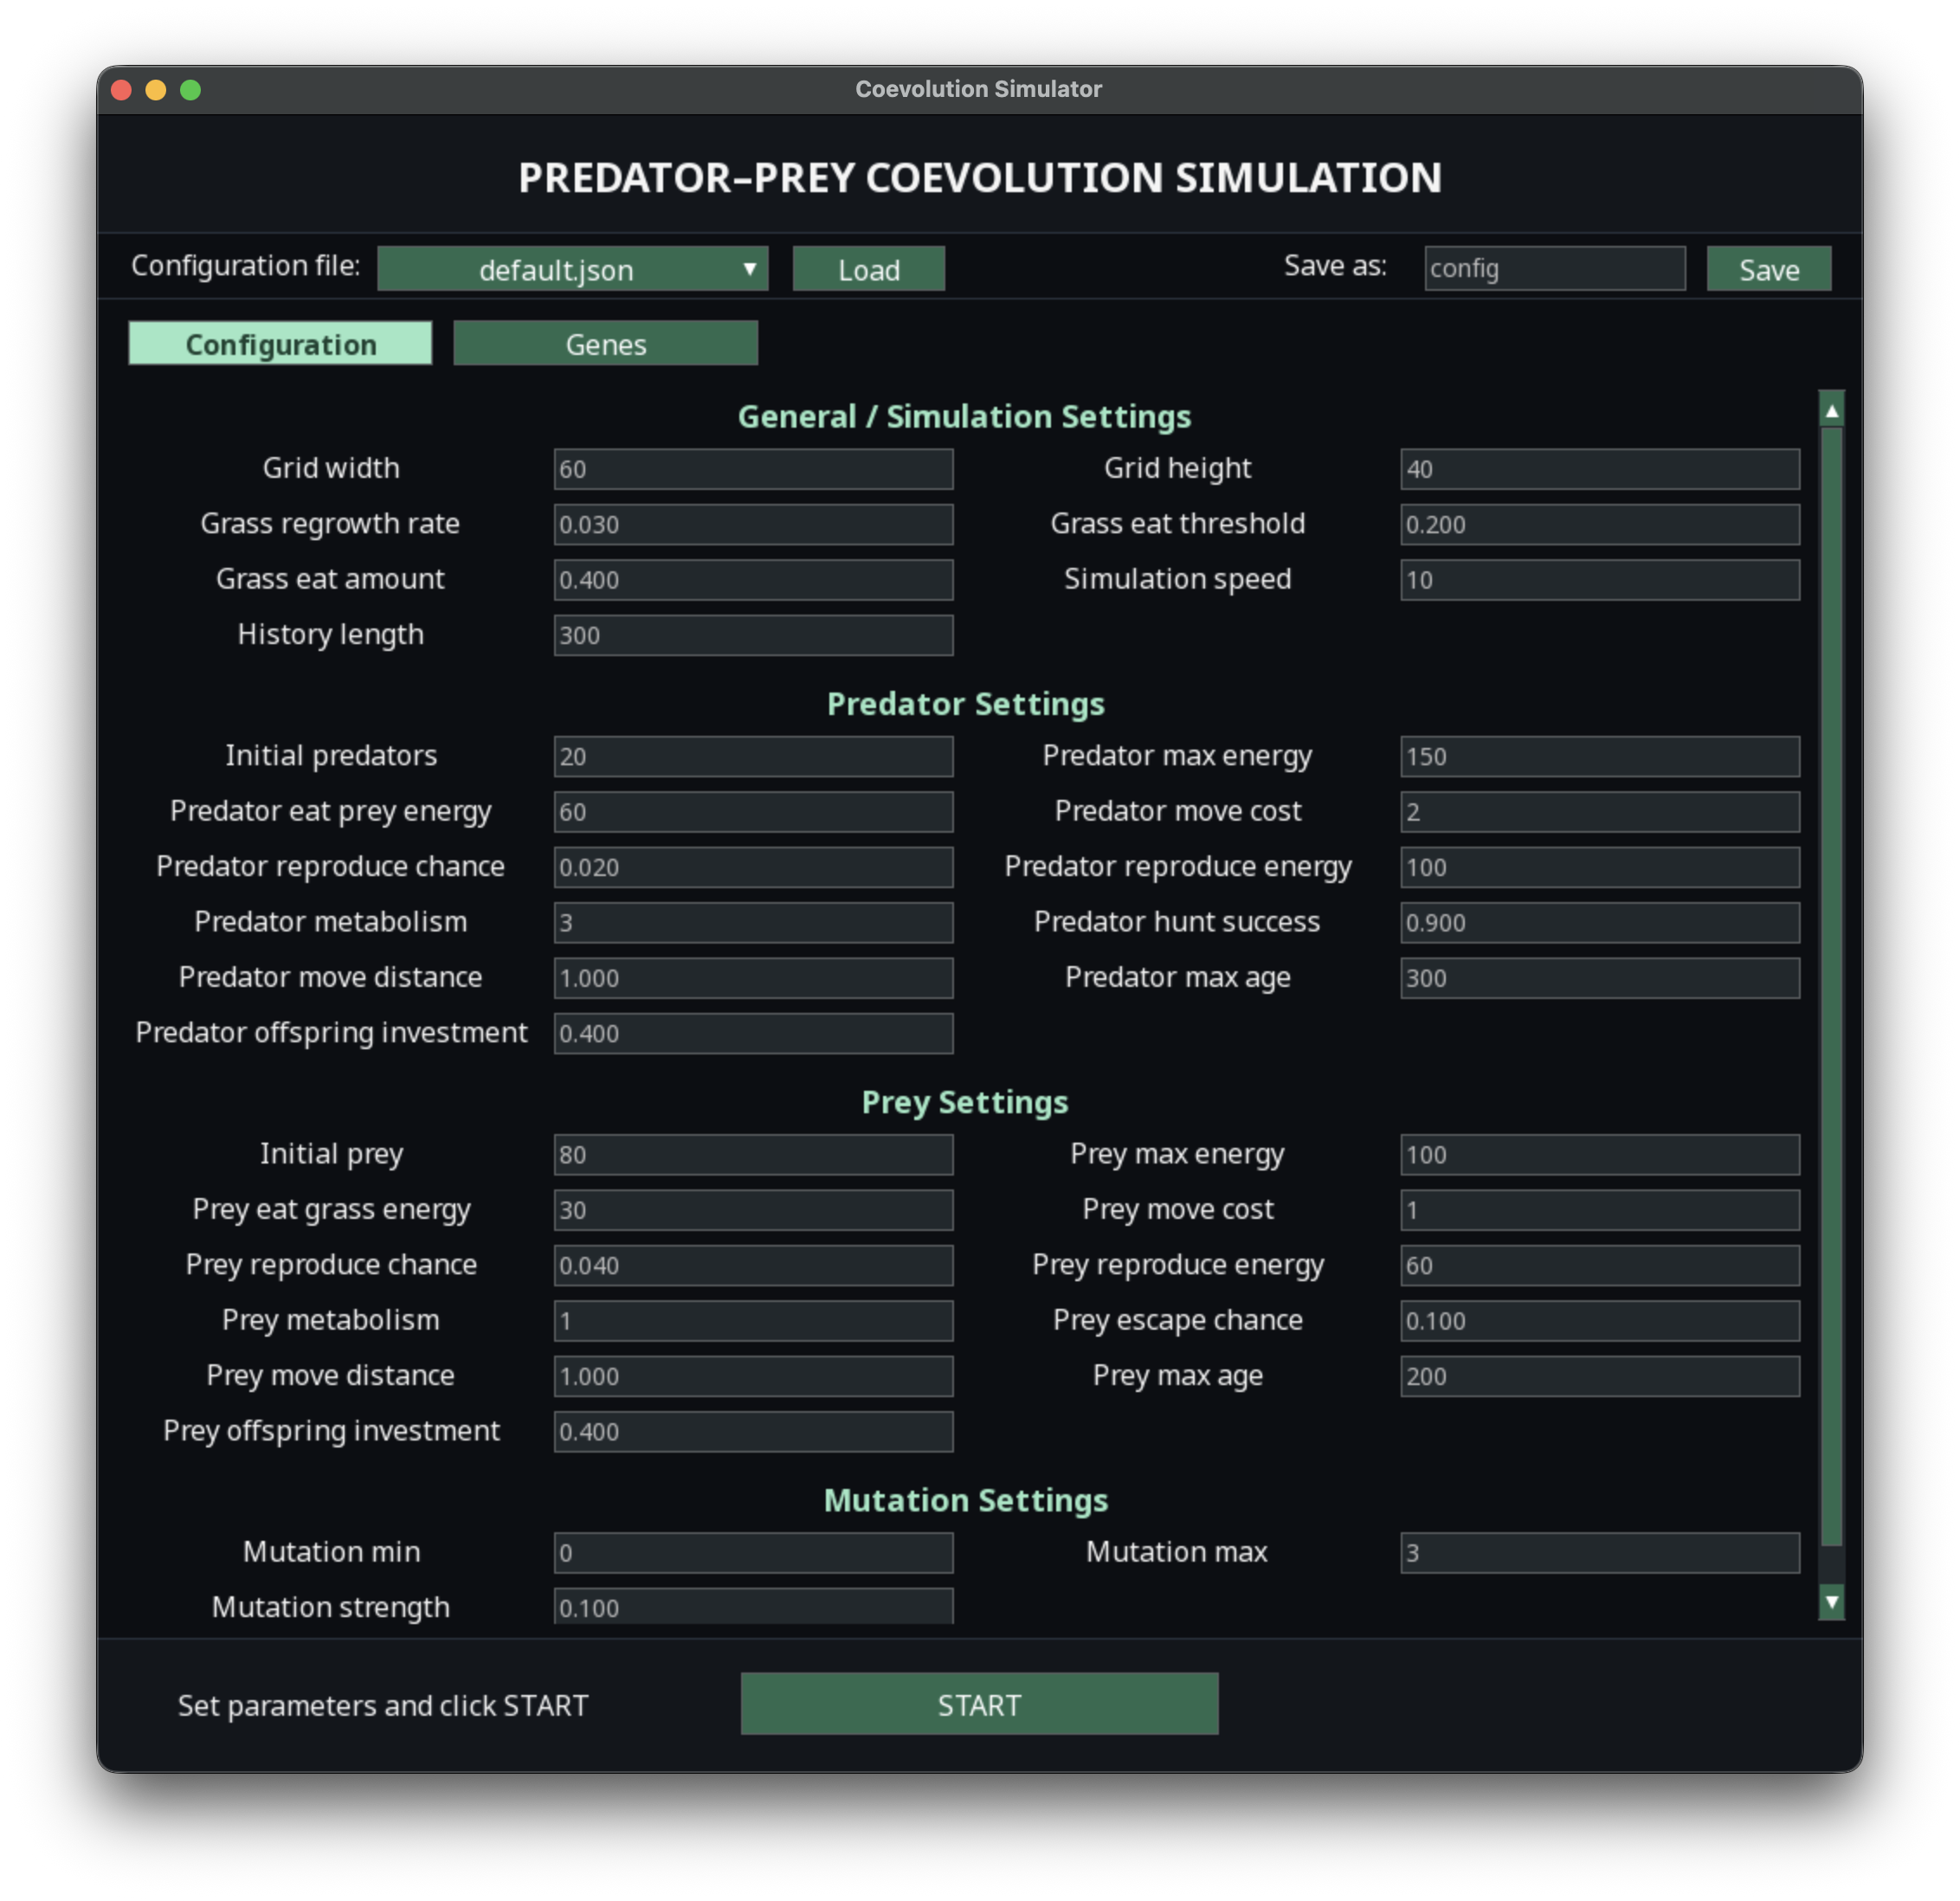
\includegraphics[width=0.85\textwidth]{figures/config_tab.png}
  \caption{Configuration screen of the simulator. The user edits ecological
  parameters grouped into general, predator, prey and mutation sections, and can
  save or load named scenarios before starting a run}
  \label{fig:config}
\end{figure}

\begin{figure}[ht]
  \centering
  \subfigure[Prey boom: many prey (blue circles) fill the grid and eat most of the grass.]{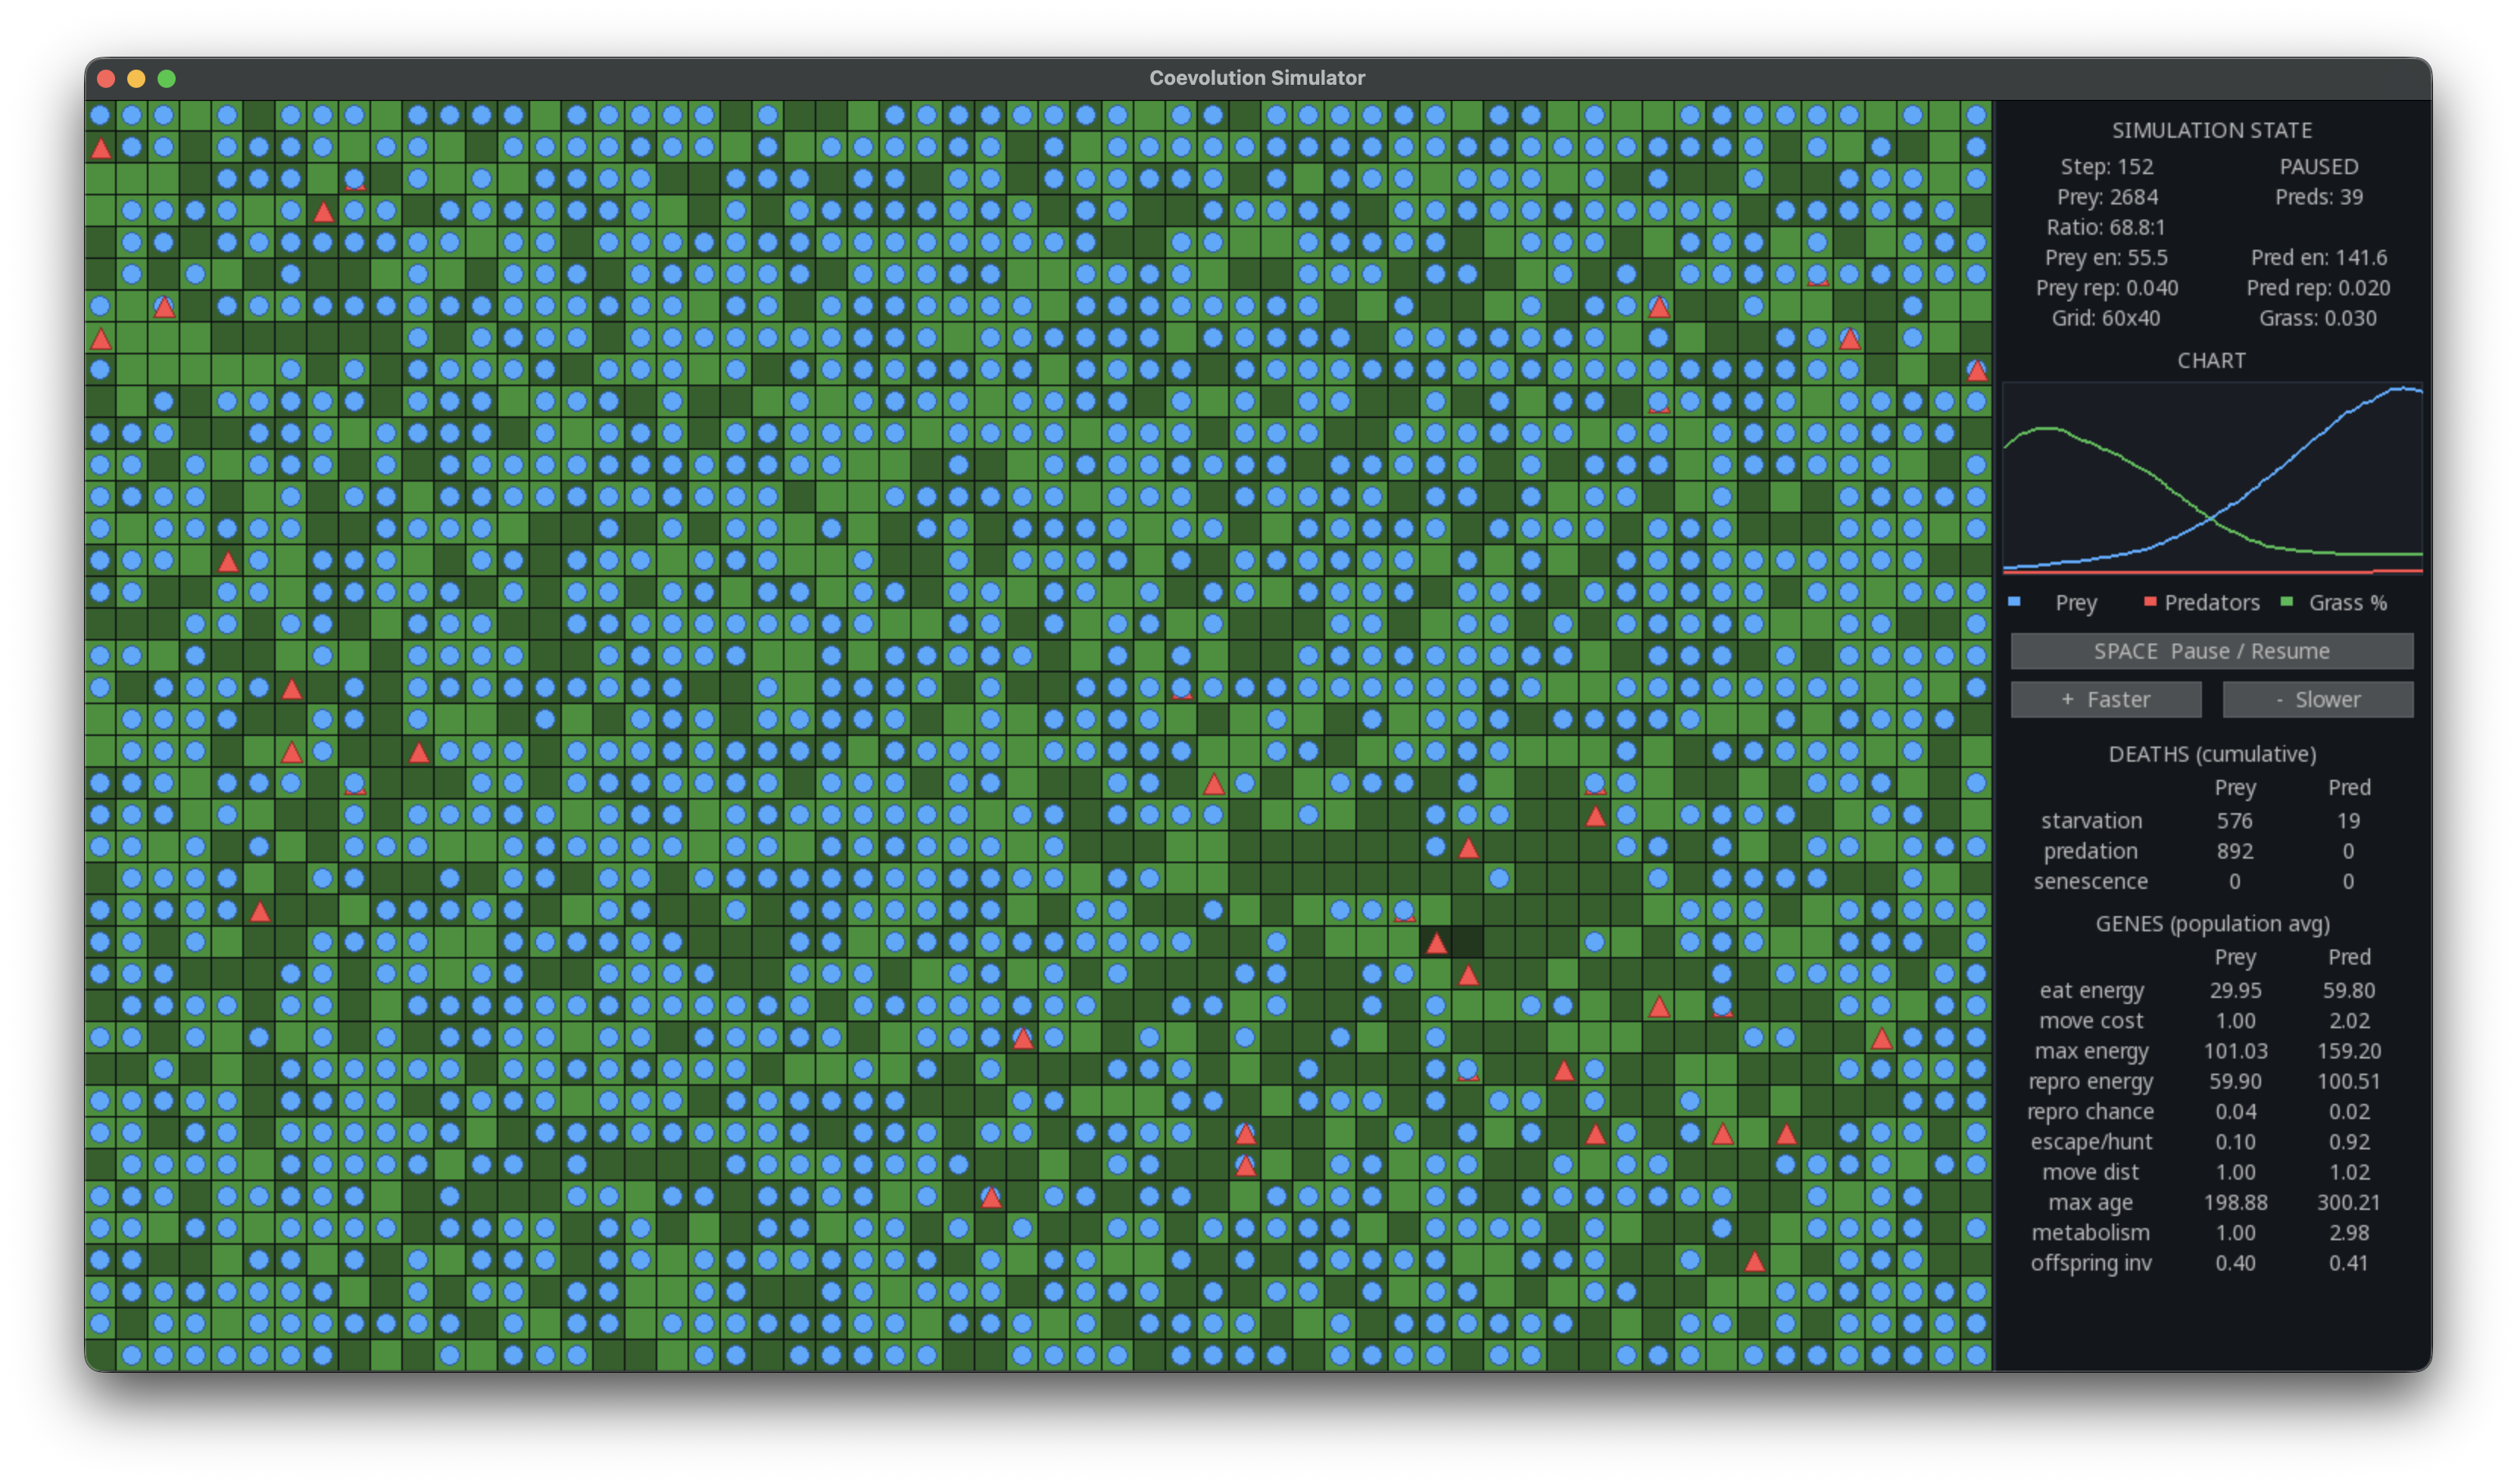
\includegraphics[width=0.46\textwidth]{figures/sim_boom.png}}
  \hfill
  \subfigure[Prey crash: many predators (red triangles) eat the prey, letting the grass grow back.]{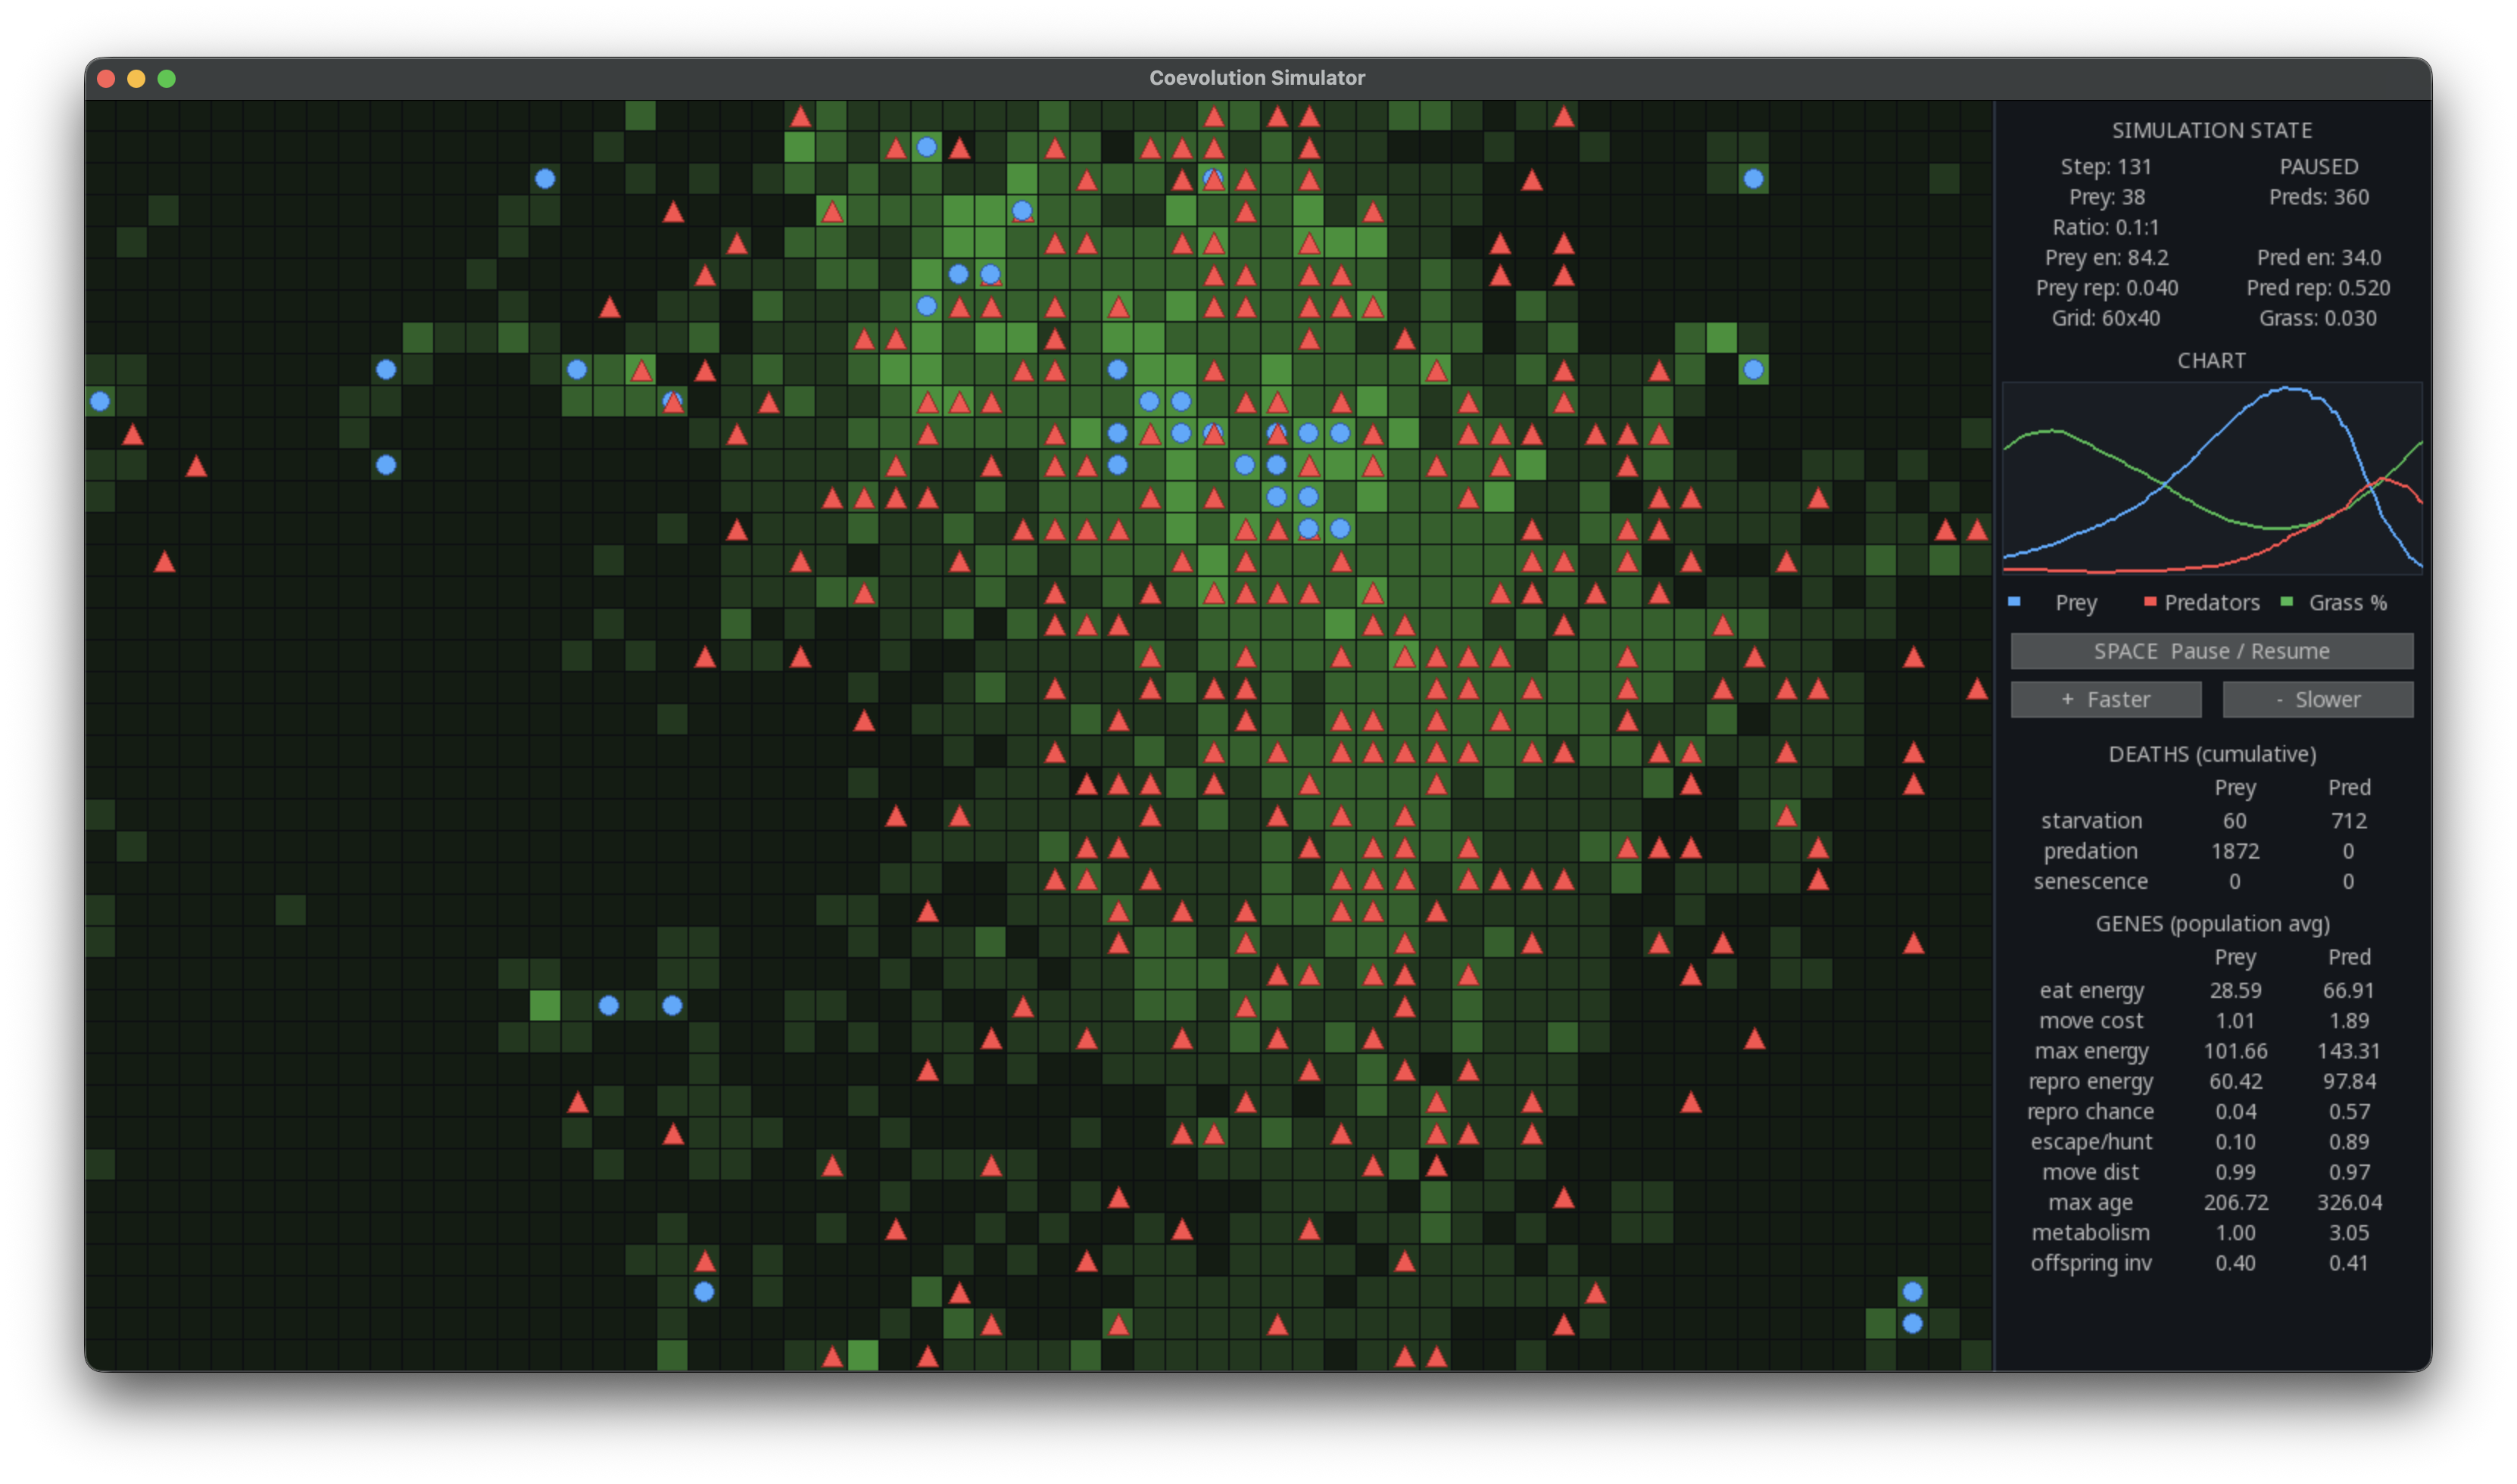
\includegraphics[width=0.46\textwidth]{figures/sim_crash.png}}
  \caption{The simulation in two phases of one population cycle. The map is on the left and live stats are on the right}
  \label{fig:sim}
\end{figure}

\begin{figure}[ht]
  \centering
  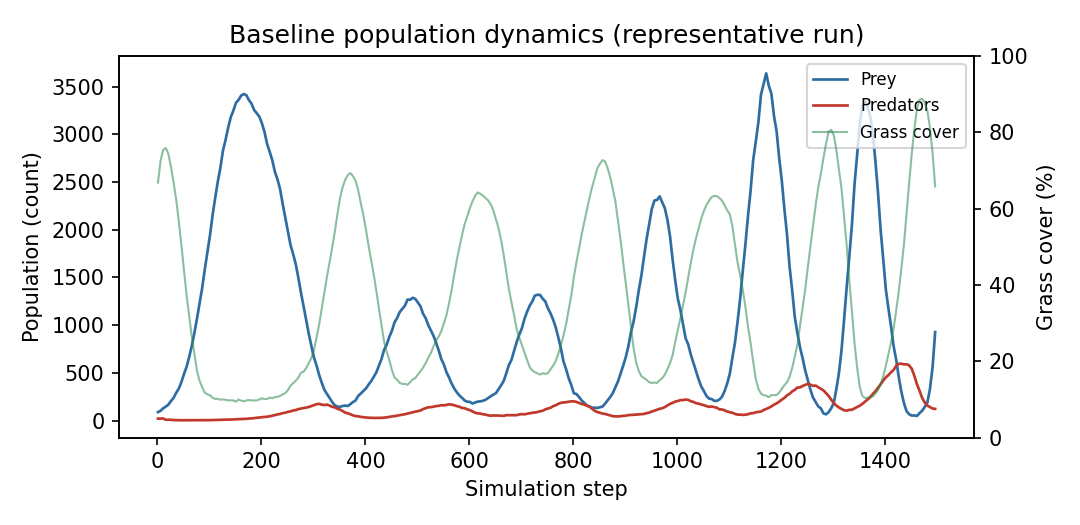
\includegraphics[width=0.9\textwidth]{figures/fig_population_dynamics.png}
  \caption{Population changes over time for a standard run ($60 \times 40$ grid, regrowth rate $0.03$, $1500$ steps). Prey and predator numbers are on the left axis; grass cover is on the right axis. Predator peaks happen just after prey peaks, showing a typical predator-prey cycle}
  \label{fig:popdyn}
\end{figure}

\begin{figure}[ht]
  \centering
  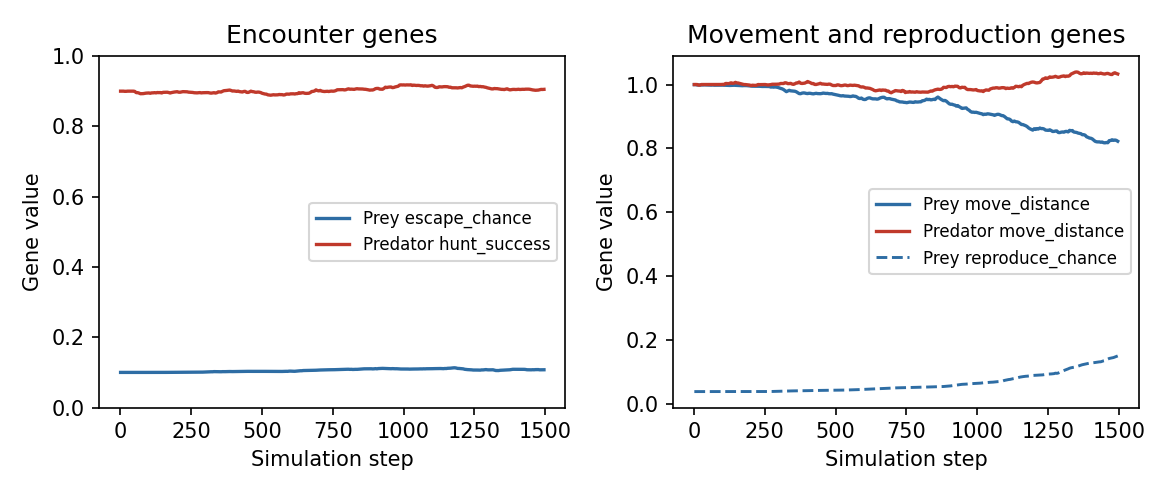
\includegraphics[width=0.95\textwidth]{figures/fig_gene_evolution.png}
  \caption{Changes in average gene values over time. Left - encounter genes (prey \texttt{escape\_chance} and predator \texttt{hunt\_success}), which barely change. Right - prey and predator \texttt{move\_distance} and prey \texttt{reproduce\_chance} (dashed line), which change a lot}
  \label{fig:genes}
\end{figure}

\begin{figure}[ht]
  \centering
  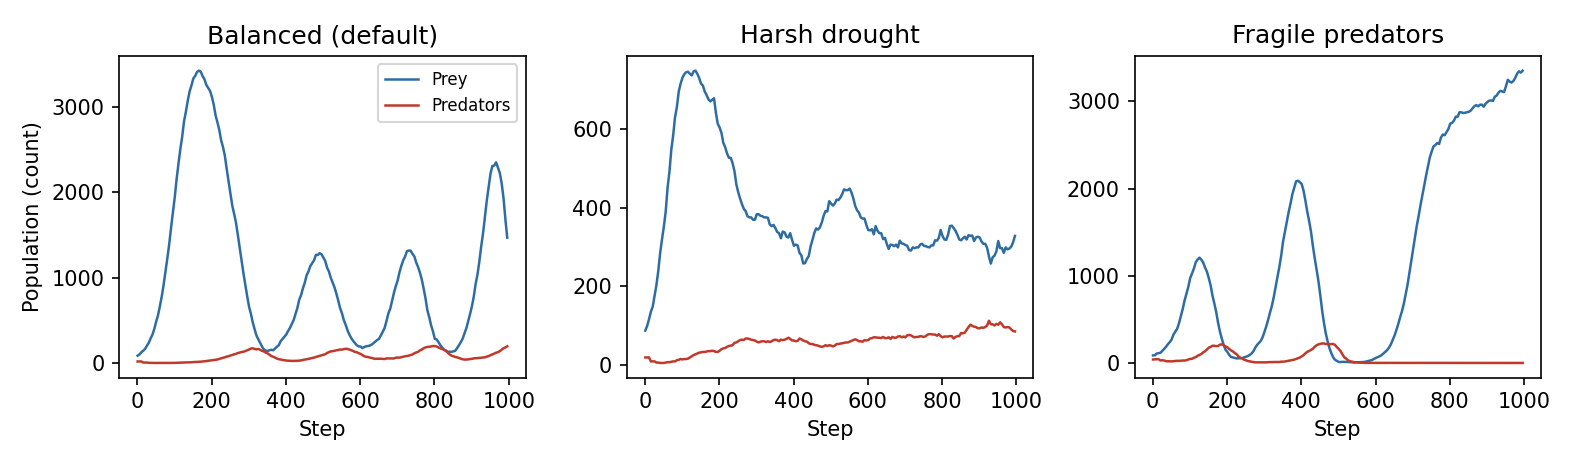
\includegraphics[width=0.98\textwidth]{figures/fig_scenarios.png}
  \caption{Population changes over time for three pre-made scenarios ($1000$ steps). The default scenario goes up and down with both species alive. The drought scenario has a much smaller and stable ecosystem. In the fragile predators scenario, predators die out around step $500$, and then the prey population grows without limit}
  \label{fig:scenarios}
\end{figure}

\subsubsection{Tables}
\label{sec:tables}

The simulation results are further detailed in four tables. Table~\ref{tab:sweep} explores the availability of resources by showing the impact of varying the grass regrowth rate. Table~\ref{tab:genes} tracks changes in the population's average genotype from the beginning to the end of the simulation. Table~\ref{tab:deaths} provides a breakdown of animal mortality by cause. Finally, Table~\ref{tab:scenarios} summarizes the outcomes of the pre-configured scenarios.

\begin{table}[ht]
  \centering
  \caption{How the grass regrowth rate affects the ecosystem ($1500$ steps). The table shows the average number of prey, predators, and grass cover. Both species survived in all cases}
  \label{tab:sweep}
  \begin{tabular}{rcrrr}
    \toprule
    Regrowth rate & Both species survived & Mean prey & Mean predators & Mean grass cover \\
    \midrule
    0.01 & Yes & 361  & 117 & 20.3\,\% \\
    0.02 & Yes & 551  & 146 & 33.2\,\% \\
    0.03 & Yes & 922  & 142 & 38.0\,\% \\
    0.05 & Yes & 1209 & 156 & 45.9\,\% \\
    0.08 & Yes & 2397 & 122 & 44.2\,\% \\
    \bottomrule
  \end{tabular}
\end{table}

\begin{table}[ht]
  \centering
  \caption{Average gene values at the start and after $1500$ steps. The last column shows the percentage change}
  \label{tab:genes}
  \begin{tabular}{llrrr}
    \toprule
    Species & Gene & Start & End & Change \\
    \midrule
    \multirow{6}{*}{Prey}
      & \texttt{reproduce\_chance}     & 0.040 & 0.151 & $+279\,\%$ \\
      & \texttt{move\_distance}        & 1.000 & 0.823 & $-18\,\%$ \\
      & \texttt{metabolism}            & 1.000 & 0.890 & $-11\,\%$ \\
      & \texttt{offspring\_investment} & 0.400 & 0.362 & $-10\,\%$ \\
      & \texttt{escape\_chance}        & 0.100 & 0.108 & $+8\,\%$  \\
      & \texttt{max\_age}              & 200   & 196   & $-2\,\%$  \\
    \midrule
    \multirow{6}{*}{Predator}
      & \texttt{metabolism}            & 3.000 & 2.534 & $-16\,\%$ \\
      & \texttt{reproduce\_chance}     & 0.020 & 0.022 & $+12\,\%$ \\
      & \texttt{max\_age}              & 300   & 277   & $-8\,\%$  \\
      & \texttt{offspring\_investment} & 0.400 & 0.426 & $+7\,\%$  \\
      & \texttt{move\_distance}        & 1.000 & 1.033 & $+3\,\%$  \\
      & \texttt{hunt\_success}         & 0.900 & 0.905 & $+1\,\%$  \\
    \bottomrule
  \end{tabular}
\end{table}

\begin{table}[ht]
  \centering
  \caption{Causes of death for prey and predators. Predators are never hunted, so their predation count is zero}
  \label{tab:deaths}
  \begin{tabular}{lrr}
    \toprule
    Cause of death & Prey & Predators \\
    \midrule
    Predation  & 82.6\,\% & 0.0\,\%  \\
    Starvation & 17.2\,\% & 98.5\,\% \\
    Senescence & 0.2\,\%  & 1.5\,\%  \\
    \midrule
    Total deaths & 433\,052 & 15\,497 \\
    \bottomrule
  \end{tabular}
\end{table}

\begin{table}[ht]
  \centering
  \caption{Results of the five pre-made scenarios after $1000$ steps. The table shows the average number of prey, predators, and grass cover, as well as whether both species survived.}
  \label{tab:scenarios}
  \begin{tabular}{lcrrr}
    \toprule
    Scenario & Both species survived & Mean prey & Mean predators & Mean grass cover \\
    \midrule
    Balanced (default) & Yes & 820  & 100 & 37.0\,\% \\
    Abundant meadow    & Yes & 1602 & 110 & 44.3\,\% \\
    Harsh drought      & Yes & 369  & 76  & 18.4\,\% \\
    Fragile predators  & No  & 2708 & 19  & 27.2\,\% \\
    Fast evolution     & Yes & 5010 & 749 & 25.8\,\% \\
    \bottomrule
  \end{tabular}
\end{table}


\subsection{Analysis and discussion}
\label{sec:discussion}

\subsubsection{Population dynamics and stability} 
The default simulation does not settle into a static balance. Instead, it produces continuous boom-and-bust cycles, as shown in Figure~\ref{fig:popdyn}. A prey boom depletes the grass and leads to a delayed increase in predators. The predators then reduce the prey population, allowing the grass to recover and starting the next cycle. This delay between prey and predator peaks resembles classic Lotka--Volterra cycles, but here it emerges purely from local interactions rather than mathematical equations. Despite these large population fluctuations, the ecosystem remains highly stable. As seen in Table~\ref{tab:sweep}, both species survived in all grass regrowth rates tested. Therefore, the ecosystem continues to cycle instead of collapsing, which answers the first research question.

\subsubsection{Effect of resource availability} 
Table~\ref{tab:sweep} shows that the rate of grass regrowth controls how many animals the environment can support. When the rate increases from 0.01 to 0.08, the average prey population grows more than six times (from 361 to 2397), and the grass cover roughly doubles. However, the predator population remains roughly the same (between 117 and 156). This difference occurs because the number of prey depend directly on food (grass). Predators, on the other hand, are limited by their high energy needs, not by a lack of prey. Therefore, having more prey leads to bigger population swings rather than many more predators. This matches the causes of death discussed next.

\subsubsection{Mortality structure} 
Table~\ref{tab:deaths} shows a clear difference between the two species. Most prey are eaten by predators (82.6\%) or die of starvation (17.2\%). Very few die of old age (0.2\%) because predators usually catch them first. Predators show the exact opposite pattern, dying almost entirely from starvation (98.5\%). In short, the number of prey is controlled by hunters, while the number of predators is limited by the finding of enough food. This creates a realistic food chain.

\subsubsection{Emergent selection and coevolution} 
Because offspring inherit the mutated genes of their parents, the population naturally evolves over time without any programmed goals \cite{dijk2010, takashi2013}. Table~\ref{tab:genes} and Figure~\ref{fig:genes} show that general survival traits (such as breeding speed and energy use) change much more than specific hunting or escaping skills. For example, prey \texttt{reproduce\_chance} jumping from 0.040 to 0.151, under heavy predator threat, the prey that survive are the ones that breed as fast as possible. This is known as an r-selected strategy: producing many offspring quickly rather than a few strong ones.

Both species also lower their \texttt{metabolism} (prey by 11\%, predators by 16\%). This saves energy and helps them survive longer between meals. Since most predators die from starvation, this is their most important adaptation. The prey also evolve a shorter \texttt{move\_distance}, saving energy and reducing the risk of falling into a predator.

In contrast, the expected "arms race" between hunters and prey is very weak. Prey \texttt{escape\_chance} increases only slightly (+8\%) and predator \texttt{hunt\_success} barely changes because it starts near its maximum limit of 1.0. In short, saving energy and breeding faster are much better survival strategies here than improving chase skills. This answers our third research question, proving that complex survival strategies can emerge naturally from simple local rules \cite{li2023}.

\subsubsection{Bundled scenarios and an extinction event} 
The project includes five pre-made scenarios to easily test different ecosystem behaviors. Their results are shown in Table~\ref{tab:scenarios} and Figure~\ref{fig:scenarios}. The \emph{abundant meadow} (plentiful grass) supports a large and lively ecosystem, while the \emph{harsh drought} (scarce grass) creates a much smaller and more stable one. In the \emph{fast evolution} scenario, a higher mutation rate causes the prey to breed so fast that their population explodes, showing how rapid mutations can destabilize the system.

The most interesting case is \emph{those of fragile predators}. Here, predators are highly deadly and prey are almost defenseless. Instead of creating a predator paradise, predators hunt, destroy their own food supply and starve to death (Table~\ref{tab:scenarios}). Once predators die out, the prey population grows without limits, as seen in the runaway blue curve in Figure~\ref{fig:scenarios}. This is exactly the kind of extinction event the project aimed to study, proving that being too good at hunting is ultimately self-defeating.

%%%%%%%%%%%%%%%%%%%%%%%%%%%%%%%%%%%%%%%%%%%%%%%%%%%%%%%%%%%%%%%%%%%%%%%%%%%%%%%
\section{Summary and conclusions}
\label{sec:summary}

This project aimed to build an accessible predator-prey simulation to study how population patterns emerge from local interactions and evolving genes. The final system meets this goal. It features a configurable ecosystem of grass, prey, and predators, where every action costs energy. It includes genetic inheritance with mutations and an interactive interface with live charts and statistics, all usable without writing any code.

The complete source code, configuration files, and the interactive environment are publicly available on GitHub at \url{https://github.com/przemuuu/System_Modeling_and_Simulation_Project}.

The experiments support three main conclusions. First, the model naturally reproduces the classic boom-and-bust cycles of predator-prey systems (Figure~\ref{fig:popdyn}), and the default ecosystem is highly stable rather than collapsing. Second, resource availability controls the ecosystem's size: faster-growing grass multiplies the prey population, while the predator population stays mostly flat due to its high energy costs. Third, population control works both ways: prey are limited by hunters, while predators are limited by starvation (Table~\ref{tab:deaths}). Under these pressures, animals naturally evolve clear survival strategies, such as faster prey breeding and lower metabolism for both species (Table~\ref{tab:genes}), without any programmed goals.

Several limitations point to future work. Testing more parameters, like mutation strength, predator efficiency, and initial populations over longer periods would make the evolutionary conclusions even stronger. Technically, the model is written in plain Python and slows down when populations reach several thousands. Optimizing the code would allow for larger maps and longer simulations. Finally, the animals genes could be expanded to include new skills, like sensing food or actively running away from threats. Adding a data export feature and a map showing where specific genes are concentrated would also help connect the evolutionary results with the visual patterns seen in Figure~\ref{fig:sim}.

%%%%%%%%%%%%%%%%%%%%%%%%%%%%%%%%%%%%%%%%%%%%%%%%%%%%%%%%%%%%%%%%%%%%%%%%%%%%%%%
\printbibliography

%%%%%%%%%%%%%%%%%%%%%%%%%%%%%%%%%%%%%%%%%%%%%%%%%%%%%%%%%%%%%%%%%%%%%%%%%%%%%%%
\end{document}
